\chapter{Tervezés, megvalósítás}

A tervezés során a legfontosabb szempont az architektúra skálázhatósága volt,
hiszen ez elengedhetetlen ahhoz, hogy az alkalmazás valóban képes legyen
elosztott működésre.

A szoftvert ezeknek a követelményeknek megfelelően akartam megtervezni,
el akartam kerülni, hogy \emph{monolitikus} alkalmazást készítsek el,
ehhez a \emph{microservice} architektúra elveit vettem figyelembe,
ami később jó döntésnek bizonyult.

A \emph{monolitikus} és a \emph{microservice} architektúra közül nem lehet
kiválasztani egyértelműen a ``jobb'' megoldást, mindkettőnek vannak előnyei
és hátrányai a másikkal szemben.

\section{Monolitikus architektúra}

Egy \emph{monolitikus} alkalmazás önálló egységet alkot, kompakt, viszonylag
kevés külső függőséggel rendelkezik. Többnyire rétegelt, vagy hexagonális
felépítéssel bír. Ez több előnnyel is jár:

\begin{itemize}
  \item A fejlesztés egyszerű, hiszen a rendelkezésre álló fejlesztőkörnyezetek
    (pl. Visual Studio) ezt a fajta architektúrát támogatják.
  \item Egyszerű az üzemeltetés, hiszen az alkalmazást könnyű deployolni, mivel
    az egyedül is képes a komplett funkcionalitást biztosítani.
  \item Több példányt elindítva a skálázás megoldható, akár automatikusan is,
    ehhez a gyakorlatban csak egy terheléselosztóra van szükség.
\end{itemize}

A hátrányai pont ezek miatt:

\begin{itemize}
  \item A komplex alkalmazások komplex fejlesztőkörnyezetet igényelnek, ami
    megnövekedett erőforrásigénnyel jár.
  \item A komplexitás következtében az alkalmazás nagyon nagy, adott esetben
    az inicializálás ideje nagyon nagyra nőhet, ami a skálázhatóságot rontja.
  \item A skálázási lehetőségek nagyon limitáltak, legtöbb esetben
    erőforráspazarlóak, hiszen az egyetlen lehetőség a több példányos futtatás.
    Ezzel nem csak a szűk keresztmetszetet jelentő komponenst duplikáltuk,
    hanem mindent.
  \item A szoros csatolás miatt megnő a \emph{vendor lock-in} veszélye,
    azaz más technológiára váltás, vagy akár csak egy verziófrissítés
    nagyon komoly kihívást jelent.
  \item Bár egy szakdolgozatban nem okoz problémát, de valódi enterprise
    környezetben egy folyamatban lévő projectbe bekapcsolódás nagyon nehézkes,
    hiszen a fejlesztőnek meg kell értenie az alkalmazást, át kell látnia azt.
\end{itemize}

\section{Microservice architektúra}

A microservice architektúra szinte pontosan az előző ellentéte.
Az egyes szoftverkomponensek önállóan is futtatható alkalmazások,
a futtatáshoz nagyon kevés erőforrásra van csak szükség, a feladatuk
ellátásához azonban szükség van sok másik komponensre.

A komponensek közti kommunikáció valamilyen jól definiált, nyelvfüggetlen
interfészen keresztül zajlik (pl HTTP fölötti JSON kommunikáció, vagy
valamilyen alacsony szintú, TCP/UDP fölött definiált protokoll).

A megoldás előnye, hogy a skálázás sokkal rugalmasabb, elegendő csak a szűk
keresztmetszetet jelentő komponenseket skálázni, így adott esetben
jelentősen kevesebb erőforrás is elengendő a megfelelő szolgáltatási
szint biztosításához.

Az architektúra további előnye, hogy technológiafüggetlen, hiszen az egyes
komponensek teljesen függetlenek egymástól, csak a megfelelő interfészeket
kell biztosítaniuk egymásnak. Egy rétegelt architektúrában ez többnyire nem
megoldható.

Természetesen hátrányok is vannak, az egyik legnyilvánvalóbb, hogy az
üzemeltetés bonyolultabb, amennyiben nem megfelelő eszközöket használunk.
A sok különálló komponens egyenkénti deployolása, illetve konfigurálása
manuálisan nagyon nehézkes, de vannak eszközök, amikkel az egész folyamat
teljesen automatizálható.

\section{Működés felvázolása}

Az alkalmazás két \verb=koa= alkalmazásból, számos apró feldolgozó folyamatból,
és a közöttük üzeneteket továbbító üzenetsorból áll (\emph{queue}),
illetve a külvilág egy \emph{reverse proxy}-n keresztül tud ezekhez hozzáférni.


\begin{itemize}
  \item Egy \verb=koa= alkalmazás bonyolítja le a felhasználóval történő
    kommunikációt (\emph{frontend}).
  \item Egy másik \verb=koa= szerver biztosítja az adatbázishoz a hálózaton
    keresztül történő hozzáférést (\emph{db}).
\end{itemize}

Az egyes alkalmazások, és a köztük lévő kapcsolatok \aref{fig:arch}.
ábrán láthatóak. A komponensek függetlenek az őket futtató környezettől,
így tetszőleges számú (fizikai vagy virtuális) hoszton futtathatóak.

\begin{figure}[h!]
  \centering
  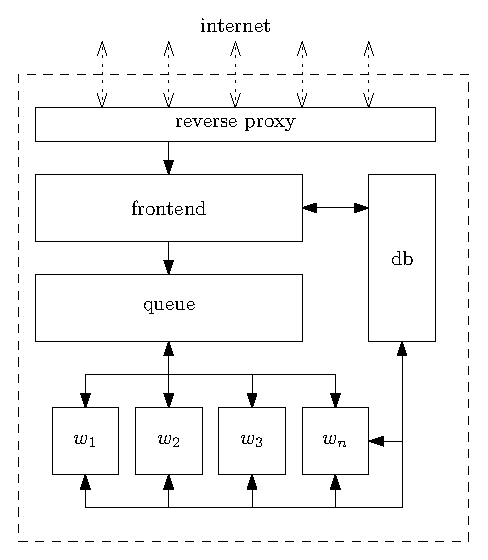
\includegraphics[width=0.6\textwidth]{figures/arch}
  \caption{Az alkalmazás architektúrája}
  \label{fig:arch}
\end{figure}

\section{Frontend alkalmazás}

A felhasználó egy webes felületet lát az alkalmazásból (a design munkákat
ezúton is köszönöm Sári Tamásnak),
a feladata, hogy egy egyszerű SPA-t (Single Page Application) biztosítson,
illetve a különböző interakciókat a megfelelő alrendszereknek továbbítsa.

A frontend szerver egy Nginx \emph{reverse proxy} mögött foglal helyet,
ami a statikus fájlokat (lefordított \verb=stylus= stílusfájlok, illetve
\verb=browserify= bundle-ök, képek) szolgál ki, minden egyéb kérést
a koa szervernek továbbít.

Alapesetben a felhasználó egy statikus HTML oldalra érkezik,
ami csak azért felelős, hogy a CSS stílusfájlok, illetve a kliensoldali JS
állományok betöltődjenek. Ezek után a felhasználó csak AJAX kéréseken keresztül
kommunikál a szerverrel.

A szerver feladata, hogy elindítsa az OAuth autentikációt, a végén keletkező
tokent az adatbázisban eltárolja, valamint beütemezze a megfelelő jobokat,
illetve ha ha ezek befejeződtek, akkor az elkészült statisztikákat
a kliensoldali alkalmazásnak eljuttassa.

\begin{figure}[h!]
  \centering
  \includegraphics[width=0.5\textwidth]{figures/frontend-1}
  \caption{Az alkalmazás kezdő képernyője}
  \label{fig:frontend-1}
\end{figure}

\begin{figure}[h!]
  \centering
  \includegraphics[width=0.5\textwidth]{figures/frontend-2}
  \caption{Az elkészült statisztika grafikonja}
  \label{fig:frontend-1}
\end{figure}

\section{Adatbázis szerver}

Az adatbázis szerver feladata az alkalmazás állapotának számon tartása.
Ezek közé tartozik az egyes \emph{business objektumok} perzisztálása,
illetve ezek menedzselése egy egyszerű REST HTTP JSON interfészen keresztül.

Az üzleti logika szempontjából releváns entitások a következők:

\begin{description}
  \item[user] a felhasználót reprezentáló objektum, a hozzá tartozó
    legfontosabb információkkal (regisztráció időpontja, e-mail cím, stb),
    illetve az elkészült statisztikákat is ebben az objektumban tárolom el.
  \item[token] az egyes Twitter API hívásokhoz szükség van a autentikációs
  tokenekre, ezeket a felhasználótól kapja meg az alkalmazás, az OAuth
  autentikációs során. Fontos számon tartani az állapotát, hányszor lett
  felhasználva, mikor lett utoljára felhasználva.
  \item[tweet] a Twitter API válaszaiból leképzett objektumok, az alkalmazás
  szempontjából az egyetlen releváns adata a tweet időpontja, hiszen ebből
  határozza meg a szoftver az ideális időpontot a tartalom publikálására.
  \item[job] az egyes elvégzendő háttérfeladatok. Az alkalmazás eltárolja a
  a teljes életciklusát, tehát hogy mikor hozták létre, mikor került egy
  feldolgozó egységhez, mikor végzett az vele. Természetesen a job állapota
  is tárolva van, ezzel a többszörös végrehajtást lehet kivédeni.
\end{description}

Egy felhasználó létrehozásakor vele együtt létrejön egy \emph{fetch-followers}
job is, ez indítja be az adott felhasználóhoz tartozó statisztikák
összegyűjtését.

Egy job létrehozásakor nem csak egy adatbázisrekord jön létre, hanem a
hozzá tartozó üzenet bekerül a várakozási sorba (ez az üzenet egyszerűen
a job azonosítóját tartalmazza), amit majd az épp aktív feldolgozóegységek
végrehajtanak.

A felhasználókhoz el van tárolva az aktív, illetve függőben lévő jobok
száma. Mivel ezeket az értékeket inkrementálni kell, amit a LevelDB atomi
műveletként nem támogat, így ezt nekem kellett megvalósítanom.
Ehhez írtam meg a \verb=co-lock= modult, ami kölcsönös kizárást biztosít
erőforrásokhoz, használata pedig a már megszokott \verb=yield= szintaktikával
lehetséges:

\begin{js}
  var lock = require('co-lock');

  var release = yield lock(resource);
  // kritikus szakasz
  yield release;
\end{js}

A háttérben a modul a \verb=resource= erőforráshoz egy zárat hoz létre,
vagy ha az már zárolva van, akkor annak a \emph{várakozási sorába} lép be,
a \verb=yield release= ezt a zárat engedi el, azaz a várakozási sorban
következő hívás hajtódik végre.

Zárak használatakor ügyelni kell a \emph{deadlock} elkerülésére.
Szerencsére az alkalmazásban máshol nem volt szükség zárakra, ezért
a deadlock nem fordulhat elő (hiszen ahhoz több erőforrásra van szükség,
az adatbázis azonban műveletenként csak egyet használ).

\section{Aszinkron üzenetsor}

A service felelőssége, hogy az egyes elvégzendő feladatokat ütemezze,
és azok a megfelelő feldolgozóegységekhez eljuttassa.

A működés során fontos, hogy az üzenetek ne vesszenek el (pl. ha a
szolgáltatás újraindul), ehhez szükség van a megfelelő kommunikációs és
tranzakciós protokollokra. Mivel ezek megvalósítása a gyakorlatban sok
körültekintést igényel, így elvetettem a saját megoldás implementálásának
lehetőségét.

A RabbitMQ szoftvert választottam a feladatra, ami az AMQP specifikációt
implementáló Erlang-alapú szoftver. Az egyes szoftverkomponensek egy RabbitMQ
szerveren keresztül kommunikálnak, így ha egy szolgáltatás rövid időre leáll,
akkor a függőben lévő üzenetek a szerveren tárolódnak (természetesen itt is
perzisztensen, így a RabbitMQ szerver leállása vagy meghibásodása esetén sem
kell tartani az adatvesztéstől).

A szerver feladata elsősorban az üzenetek továbbítása, azonban az üzenetsor
működésének jellegét kihasználva egy \emph{resource pool}-t is megvalósítottam
vele. Az egyes feladatok elvégzéséhez szükség van \emph{tokenekre}, melyek
segítségével autentikált Twitter API hívások végezhetők, mivel azonban ezek
használata erősen korlátozott (adott időintervallumban csak bizonyos számú
API hívás végezhető el), így meg kell akadályozni, hogy az egyes tokenek
``kimerüljenek'', azaz kölcsönös kizárást kell biztosítani hozzájuk,
azokat csak meghatározott időközönként lehet újra felhasználni.
A vázlatos működés \aref{fig:queue}. ábrán látható.

\begin{figure}[h!]
  \centering
  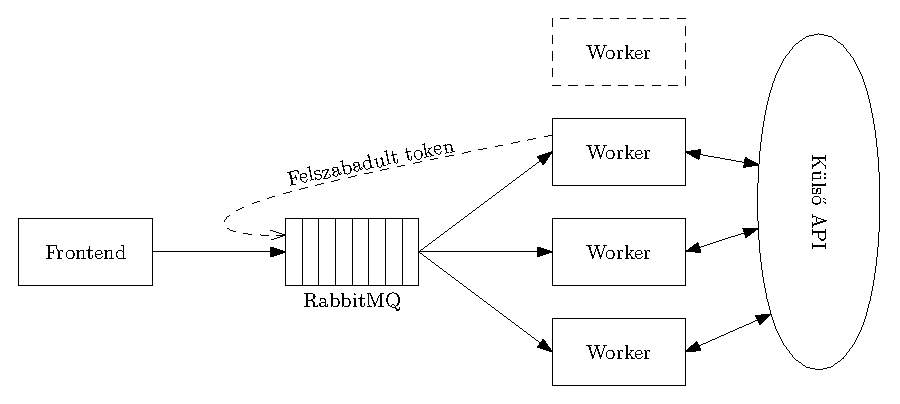
\includegraphics[width=0.95\textwidth]{figures/queue}
  \caption{Az üzenetsor szerepe az alkalmazásban}
  \label{fig:queue}
\end{figure}

\subsection{AMQP}

Az AMQP (Advanced Message Queuing Protocol) egy rugalmas protokoll üzenetek
változatos minták szerinti továbbítására. A \emph{termelők} a szerverhez
kapcsolódva egy \emph{exchange}-ben publikálják az üzenetüket,
a szerver pedig az üzenet \emph{routing key}-e
(és az aktuális \emph{exchange-queue bindingok}) alapján továbbítja a
megfelelő \emph{queue(k)}-ba. A \emph{fogyasztók} az egyes queue-kra
iratkoznak fel, a szerver pedig továbbítja az üzenetet egy (vagy több)
fogyasztónak.

Az elkészült alkalmazás nem használ bonyolult mintákat, minden üzenet
az alapértelmezett exchangen keresztül publikálódik, a routing key pedig
megegyezik a queue nevével, ami pedig az adott feladat nevével egyezik meg,
így az egyszerűség kedvéért a továbbiakban az üzenet publikálás alatt
azt lehet érteni, hogy megérkezik a routing key-nek megfelelő queue-ba az
üzenet.

\subsection{Resource pool}

Az egyes tokenek felhasználása korlátozott, így a befejezett feladat után
nem szabad azt rögtön visszarakni a pool-ba, hanem bizonyos ideig
``várakoztatni'' kell.

Ezt egy közbenső queue beiktatásával oldom meg. Az AMQP protokol támogatja,
hogy az egyes üzenetekhez TTL-t (Time to Live) rendeljünk.
Ha az üzenetet nem sikerült ezen idő alatt eljuttatni egy fogyasztóhoz,
akkor automatikusan \emph{dead} állapotú lesz. Ha a queue-nak beállítunk
ún. \emph{dead-letter-exchange}-t, akkor ezek az üzenetek kiürülnek az
üzenetsorból, és újra publikálódnak a megadott exchange-n, a megadott
routing key-el (\emph{dead-letter-routing-key}).

Ezt kihasználva, használat után az egyes tokenek egy olyan queue-ba kerülnek,
aminek nincsenek fogyasztói, ezért a megfelelő idő eltelte után újra
visszakerülnek a pool-ba. A működés \aref{fig:pool}. ábrán látható.

\begin{figure}[h!]
  \centering
  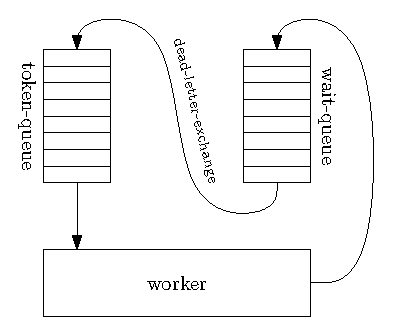
\includegraphics[width=0.6\textwidth]{figures/pool}
  \caption{Resource pool megoldás}
  \label{fig:pool}
\end{figure}

Mivel a TTL a queue-ra nézve állandó (létezik az üzenetre értelmezett TTL is,
de az nem használható az általam elérni kívánt funkcionalitáshoz), így
minden TTL-hez külön queue-t kell deklarálni.
Erre hoztam létre az \verb=amqp-schedule= modult. A könyvtár egy egyszerű
interfésszel elrejti előlünk ezt az ideiglenes üzenetsort:

\begin{js}
  var scheduler = require('amqp-schedule');
  var publish = scheduler(conn); // conn: amqp kliens objektum

  publish(exchange, key, message, delay, opts, cb);
  // vagy
  publish(exchange, key, message, date, opts, cb);
\end{js}

A késleltetés a \verb=delay= paraméterrel szabályozható, vagy konkrét időpont
(\verb=date=) is megadható. A háttérben egy speciálisan elnevezett
queue jön létre, ami a megfelelő \emph{dead-letter-exchange},
\emph{dead-letter-routing-key} és \emph{message-ttl} paraméterekkel rendelkezik,
azaz a megadott idő után az üzenet automatikusan a cél queue-ba kerül.
Mivel az eltérő időzítések új üzenetsorokat hoznak létre, így
a létrejött ideiglenes queue-k rendelkeznek \emph{expires} paraméterrel,
ami azt szabja meg, hogy mennyi \emph{idle} idő (üresjáratban töltött)
után szűnjenek meg maguktól. Így a szerver védve van attól, hogy a már nem
használt, üres üzenetsorok erőforrásokat foglaljanak.

\section{Háttérfolyamatok}

\begin{figure}[h!]
  \centering
  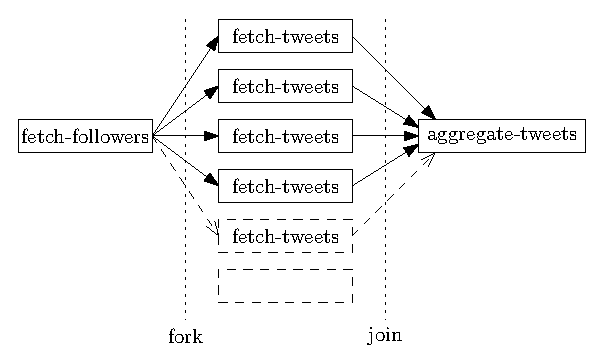
\includegraphics[width=0.75\textwidth]{figures/workflow}
  \caption{Az alkalmazásban lévő háttérfolyamatok összefüggései}
  \label{fig:workflow}
\end{figure}

Az egyes háttérfolyamatok egyszerű Node.JS alkalmazások, amik csatlakoznak
a RabbitMQ szerverhez, és egy adott típusú feladatot végeznek el.

Tetszőleges számú példány elindítható, a kommunikáció hálózaton keresztül
zajlik, így amíg hozzáférnek az üzenetsorhoz, illetve az adatbázishoz,
addig lényegtelen, hogy milyen környezetben futnak.

Alapvetően három fajta feladatot definiáltam, ezek összefüggései
\aref{fig:workflow}. ábrán láthatóak. A feladatok végrehajtásának sorrendje
nem kötött, azonban az egyes folyamatoknam szükségük van egy ponton
szinkronizációra, ennek megoldása nem triviális feladat.

\subsection{Job elosztás}

Az egyes elvégzendő feladatokat a RabbitMQ osztja szét a kliensek között,
akik egymástól teljesen függetlenül képesek működni párhuzamosan,
akár több futtató gépen is.

Az AMQP protokoll támogatja az üzenetek kézbesítésének visszaigazolásos módját,
azaz egy üzenet a célba juttatás esetén csak \emph{unacked} állapoba kerül,
azt a kliensek kell visszaigazolnia. Ezt a kliens az adott feladt elvégzése
után teszi meg, ha a feladatot nem sikerül elvégezni (mert a kliens ezt
explicit kijelenti, vagy a kapcsolat a klienssel megszakad), akkor
az üzenet automatikusan újraütemeződik.

Az AMQP Node.JS binding nem támogatja az üzenetek egyesével történő
elfogyasztását, így az általam használt megoldás egy feliratkozásból,
és egy leiratkozásból áll:

\begin{js}
function* peek(queue) {
  var done;
  var tag;
  queue.subscribe({
    ack: true,
    prefetchCount: 1,
  }, function(message, headers, deliveryInfo, job) {
    queue.unsubscribe(tag).addCallback(function() {
      done(null, {
        message: message,
        headers: headers,
        deliveryInfo: deliveryInfo,
        job: job,
      });
    });
  }).addCallback(function (ok) {
    tag = ok.consumerTag;
  });
  return yield function(cb) {
    done = cb;
  };
}
\end{js}

A feliratkozáskor a kliens egy ún. \emph{consumer tag}-et kap,
ami a feliratkozást azonosítja. Az üzenetek \emph{ack} módban érkeznek,
azaz amíg \verb=prefetchCount= számú üzenet nincs visszaigazolva,
addig a nem kap több üzenetet a kliens.

Ha az első üzenet megérkezett, akkor a kliens az eltárolt consumer tag
alapján elvégzi a leiratkozást, és a hívónak visszaadja a kapott üzenetet,
illetve a hozzá tartozó metaadatokat. Ha a hívó elvégezte a feladatát,
a \verb=job.acknowledge()= metódussal visszaigazolja az üzenetet,
vagy a \verb=job.reject(requeue)=-tel eldobja (és a paraméter értékétől
függően újra beálltja az üzenetsorba).

\subsection{fetch-followers}

A feldolgozás első lépése, hogy a felhasználó követőit lekérdezzük a Twitter
API-ból.

Az API válasz hatására minden egyes követőhöz hozzá kell rendelni
(és beütemezni) egy \emph{fetch-tweets} feladatot,
ami majd az egyes felhasználók tweetjeit fogja megszerezni.

Egy API kérés maximum 1500 követőt képes visszaadni, így ennél nagyobb
mennyiségnél újabb \emph{fetch-followers} feladatot kell beütemezni,
így a \emph{fetch-followers} rekurzívan szerzi meg a felhasználó követőit.

\subsection{fetch-tweets}

A \emph{fetch-tweets} egy adott felhasználó legutolsó tweetjeit kérdezi le,
egy adott időponttól kezdve. A tervezés során úgy határoztam, hogy az egyes
felhasználóknak csak az utolsó két hétben publikált tweetjeit kérdezem le,
vagy amennyit a rendszer megenged (3200 tweet, szerencsére ez minden
esetben elegendőnek bizonyult).
Kezdetben a legutolsó 200 tweetet kérdezi le a rendszer,
majd ha ezek közül egyik tweet sem régebbi 2 hétnél,
akkor a készít egy új \emph{fetch-tweets} jobot, ami a legrégebbi
(de még mindig két hétnél frissebb) tweet előtti üzeneteket tölti le.
Így előbb-utóbb rekurzív módon minden szükséges tweet letöltésre kerül.

\subsection{aggregate-tweets}

Ha az adatok begyűjtése megtörtént, akkor a rendszer elvégzi az összegyűjtött
tweetek aggregálását. A folyamat egyrészt detektálja, hogy valóban el kell-e
végezni az aggregálást (azaz a felhasználónál nem maradt már \emph{pending}
állapotú feladat): ha még további adatok letöltése szükséges,
akkor befejezi a futást.
Amint az utolsó job is lefutott, megtörténik a tényleges aggregálás.
Ehhez le kell kérdezni az adatbázisból az összegyűjtött tweeteket, majd
azokat csoportosítani a létrehozásuk ideje alapján, végül az ezekbe a
csoportokba eső üzeneteket kell megszámolni. Az eredményt el kell tárolni,
hogy azt a frontend alkalmazás a felhasználónak később meg tudja mutatni.

\section{Naplózás}

A naplózást minden rendszer saját hatáskörében végzi el, azonban azokat
egy közös helyre (InfluxDB) is beteszi. Így az adatok központilag elemezhetők,
de lebonthatóak alkalmazásokra, hosztokra, folyamatokra.

\subsection{HTTP kérés naplózás}

A frontend szerver egyszerűen a beérkező HTTP kéréseket naplózza, ezek
válaszidejét méri. Ez a gyakorlatban az OAuth-tal összefüggő kéréseket
jelenti.

\subsection{Adatbázis naplózás}

Az adatbázis külön naplóz minden adathozzáférést, annak típusa szerint
csoportosítva (írás, olvasás), illetve az erőforrás típusa (tweet, user, stb.)
alapján. Ezen felül a HTTP interfészének válaszidejét is méri, így
külön-külön mérhető az adatbázis, illetve a szerver válaszideje
(a szerver válaszideje ekkor az adatbázis és a
HTTP szerver \emph{overhead}jének összege).

\subsection{Háttérfolyamatok}

Az egyes végrehajtó folyamatok is monitorozzák az általuk végrehajtott
feladatokat

\begin{itemize}
  \item Mennyi idő alatt hajtotta végre az adott feladatot
  \item Mekkora volt a Twitter API válaszideje
  \item Mennyi időt töltött a várakozási sorban, amíg sorra került
  \item Hiba esetén naplózni kell a hiba eredetét (adatbázishiba,
    vagy a Twitter hibája)
\end{itemize}

A feldolgozás során a Twitter számos hibát generál. Ezek túlnyomó többsége
a privát Twitter felhasználók miatt van: az ő tweetjeit csak bizonyos
emberek láthatják (akiknek előzetesen jóváhagyta), így ezeket az üzeneteket
az API-ból sem tudjuk elérni. Ilyenkor jobb megoldás híján az adott
\emph{fetch-tweets} jobot befejezettnek tekintjük.

Fel kell készülni az olyan hibákra is, hogy az API (vagy éppen az adatbázis)
elérhetetlen: ilyenkor a jobot nem szabad lezárni, újra be kell ütemezni.
Ez praktikusan egy \verb=job.reject(true)= hívással történik meg, azaz
a feladat visszakerül a feldolgozási sor elejére.

